\documentclass[11pt,a4paper]{article}
\newcommand{\intestazione}{Dimero di spin --- 4. Correlatori}
% =====================================================================
%  Preambolo comune ai documenti sul dimero (serie "che cosa abbiamo fatto")
%  Incluso con % =====================================================================
%  Preambolo comune ai documenti sul dimero (serie "che cosa abbiamo fatto")
%  Incluso con % =====================================================================
%  Preambolo comune ai documenti sul dimero (serie "che cosa abbiamo fatto")
%  Incluso con \input{preambolo_dimero} subito dopo \documentclass.
% =====================================================================
\usepackage[T1]{fontenc}
\usepackage[utf8]{inputenc}
\usepackage[main=italian,provide=*]{babel}
\usepackage{amsmath,amssymb,mathtools}
\usepackage{graphicx}
\usepackage{booktabs}
\usepackage{colortbl}
\usepackage{xcolor}
\usepackage{geometry}
\usepackage{placeins}
\usepackage{caption}
\usepackage{enumitem}
\usepackage{fancyhdr}
\usepackage{needspace}
\usepackage{tikz}
\usetikzlibrary{arrows.meta,positioning,shapes.geometric,calc,fit,backgrounds}
\usepackage{hyperref}
\hypersetup{colorlinks=true,linkcolor=blu,citecolor=blu,urlcolor=blu}

\geometry{margin=2.5cm}

% --- colori coerenti con quelli delle figure (palette Okabe-Ito)
\definecolor{blu}{HTML}{0072B2}
\definecolor{arancio}{HTML}{E69F00}
\definecolor{verdes}{HTML}{009E73}
\definecolor{rossos}{HTML}{D55E00}
\definecolor{violas}{HTML}{CC79A7}
\definecolor{grigetto}{HTML}{E8E8E8}

\captionsetup{font=small,labelfont=bf,width=0.92\textwidth}

\pagestyle{fancy}
\fancyhf{}
\fancyhead[L]{\small\itshape\intestazione}
\fancyhead[R]{\small\thepage}
\renewcommand{\headrulewidth}{0.3pt}

% --- notazione
\newcommand{\ket}[1]{\lvert #1\rangle}
\newcommand{\bra}[1]{\langle #1 \rvert}
\newcommand{\media}[1]{\langle #1 \rangle}
\newcommand{\vs}[1]{\mathbf{s}_{#1}}

% --- riquadro "in una riga": il messaggio da portare a casa
\newcommand{\messaggio}[1]{%
  \begin{center}
  \begin{minipage}{0.93\textwidth}
  \setlength{\fboxsep}{9pt}%
  \colorbox{grigetto}{\begin{minipage}{\dimexpr\textwidth-2\fboxsep}
  \small\textbf{In una riga.}\enspace #1
  \end{minipage}}
  \end{minipage}
  \end{center}
}

% --- riquadro "come lo sappiamo": la verifica numerica dietro un'affermazione
\newcommand{\verifica}[1]{%
  \begin{center}
  \begin{minipage}{0.93\textwidth}
  \small\textcolor{verdes}{\rule{2.2em}{1.1pt}}\enspace
  \textcolor{verdes}{\textbf{Come lo sappiamo.}}\enspace #1
  \end{minipage}
  \end{center}
  \medskip
}
 subito dopo \documentclass.
% =====================================================================
\usepackage[T1]{fontenc}
\usepackage[utf8]{inputenc}
\usepackage[main=italian,provide=*]{babel}
\usepackage{amsmath,amssymb,mathtools}
\usepackage{graphicx}
\usepackage{booktabs}
\usepackage{colortbl}
\usepackage{xcolor}
\usepackage{geometry}
\usepackage{placeins}
\usepackage{caption}
\usepackage{enumitem}
\usepackage{fancyhdr}
\usepackage{needspace}
\usepackage{tikz}
\usetikzlibrary{arrows.meta,positioning,shapes.geometric,calc,fit,backgrounds}
\usepackage{hyperref}
\hypersetup{colorlinks=true,linkcolor=blu,citecolor=blu,urlcolor=blu}

\geometry{margin=2.5cm}

% --- colori coerenti con quelli delle figure (palette Okabe-Ito)
\definecolor{blu}{HTML}{0072B2}
\definecolor{arancio}{HTML}{E69F00}
\definecolor{verdes}{HTML}{009E73}
\definecolor{rossos}{HTML}{D55E00}
\definecolor{violas}{HTML}{CC79A7}
\definecolor{grigetto}{HTML}{E8E8E8}

\captionsetup{font=small,labelfont=bf,width=0.92\textwidth}

\pagestyle{fancy}
\fancyhf{}
\fancyhead[L]{\small\itshape\intestazione}
\fancyhead[R]{\small\thepage}
\renewcommand{\headrulewidth}{0.3pt}

% --- notazione
\newcommand{\ket}[1]{\lvert #1\rangle}
\newcommand{\bra}[1]{\langle #1 \rvert}
\newcommand{\media}[1]{\langle #1 \rangle}
\newcommand{\vs}[1]{\mathbf{s}_{#1}}

% --- riquadro "in una riga": il messaggio da portare a casa
\newcommand{\messaggio}[1]{%
  \begin{center}
  \begin{minipage}{0.93\textwidth}
  \setlength{\fboxsep}{9pt}%
  \colorbox{grigetto}{\begin{minipage}{\dimexpr\textwidth-2\fboxsep}
  \small\textbf{In una riga.}\enspace #1
  \end{minipage}}
  \end{minipage}
  \end{center}
}

% --- riquadro "come lo sappiamo": la verifica numerica dietro un'affermazione
\newcommand{\verifica}[1]{%
  \begin{center}
  \begin{minipage}{0.93\textwidth}
  \small\textcolor{verdes}{\rule{2.2em}{1.1pt}}\enspace
  \textcolor{verdes}{\textbf{Come lo sappiamo.}}\enspace #1
  \end{minipage}
  \end{center}
  \medskip
}
 subito dopo \documentclass.
% =====================================================================
\usepackage[T1]{fontenc}
\usepackage[utf8]{inputenc}
\usepackage[main=italian,provide=*]{babel}
\usepackage{amsmath,amssymb,mathtools}
\usepackage{graphicx}
\usepackage{booktabs}
\usepackage{colortbl}
\usepackage{xcolor}
\usepackage{geometry}
\usepackage{placeins}
\usepackage{caption}
\usepackage{enumitem}
\usepackage{fancyhdr}
\usepackage{needspace}
\usepackage{tikz}
\usetikzlibrary{arrows.meta,positioning,shapes.geometric,calc,fit,backgrounds}
\usepackage{hyperref}
\hypersetup{colorlinks=true,linkcolor=blu,citecolor=blu,urlcolor=blu}

\geometry{margin=2.5cm}

% --- colori coerenti con quelli delle figure (palette Okabe-Ito)
\definecolor{blu}{HTML}{0072B2}
\definecolor{arancio}{HTML}{E69F00}
\definecolor{verdes}{HTML}{009E73}
\definecolor{rossos}{HTML}{D55E00}
\definecolor{violas}{HTML}{CC79A7}
\definecolor{grigetto}{HTML}{E8E8E8}

\captionsetup{font=small,labelfont=bf,width=0.92\textwidth}

\pagestyle{fancy}
\fancyhf{}
\fancyhead[L]{\small\itshape\intestazione}
\fancyhead[R]{\small\thepage}
\renewcommand{\headrulewidth}{0.3pt}

% --- notazione
\newcommand{\ket}[1]{\lvert #1\rangle}
\newcommand{\bra}[1]{\langle #1 \rvert}
\newcommand{\media}[1]{\langle #1 \rangle}
\newcommand{\vs}[1]{\mathbf{s}_{#1}}

% --- riquadro "in una riga": il messaggio da portare a casa
\newcommand{\messaggio}[1]{%
  \begin{center}
  \begin{minipage}{0.93\textwidth}
  \setlength{\fboxsep}{9pt}%
  \colorbox{grigetto}{\begin{minipage}{\dimexpr\textwidth-2\fboxsep}
  \small\textbf{In una riga.}\enspace #1
  \end{minipage}}
  \end{minipage}
  \end{center}
}

% --- riquadro "come lo sappiamo": la verifica numerica dietro un'affermazione
\newcommand{\verifica}[1]{%
  \begin{center}
  \begin{minipage}{0.93\textwidth}
  \small\textcolor{verdes}{\rule{2.2em}{1.1pt}}\enspace
  \textcolor{verdes}{\textbf{Come lo sappiamo.}}\enspace #1
  \end{minipage}
  \end{center}
  \medskip
}


\title{\bfseries Misurare una correlazione fra due istanti diversi\\[2pt]
\large Documento 4 --- correlatori dinamici e circuito con qubit ausiliario}
\author{Samuele Schiavi \\ \small Tesi triennale in Fisica, Università di Parma
--- Relatore: Prof.\ Alessandro Chiesa}
\date{}

\begin{document}
\maketitle
\thispagestyle{fancy}

\section{Che cosa vogliamo misurare, e perché non si può misurare direttamente}

La quantità di interesse è
\begin{equation}
C_{ij}^{\alpha\beta}(t) \;=\;
\bra{\psi_0}\,\sigma_i^\alpha(t)\,\sigma_j^\beta(0)\,\ket{\psi_0},
\qquad \alpha,\beta\in\{x,y,z\},\quad i,j\in\{1,2\}.
\end{equation}
In parole: si perturba lo spin $j$ lungo la direzione $\beta$ all'istante zero,
si lascia evolvere il sistema, e si guarda quanto quella perturbazione si
ritrova sullo spin $i$ lungo la direzione $\alpha$ al tempo $t$. È la grandezza
che collega la simulazione alla misura sperimentale: la sua trasformata di
Fourier è ciò che si osserva in una misura di scattering di neutroni su una
molecola magnetica.

Il problema pratico è che questa non è la media di un osservabile. Il prodotto
$\sigma_i^\alpha(t)\,\sigma_j^\beta(0)$ non è hermitiano --- il suo valore è un
numero complesso --- e nessuna misura proiettiva restituisce direttamente parte
reale e parte immaginaria di un oggetto simile.

\messaggio{Le osservabili a un corpo si misurano direttamente. Una correlazione
a due tempi no: serve un qubit in più che non rappresenta alcuno spin fisico, e
funziona da strumento di misura.}

\section{Il circuito: l'ancilla come interferometro}

Lo schema è un test di Hadamard. Il qubit ausiliario viene messo in
sovrapposizione, e le operazioni sul registro fisico vengono condizionate al suo
stato: nel ramo $\ket{0}$ il sistema fa una cosa, nel ramo $\ket{1}$ un'altra. I
due rami interferiscono, e la misura dell'ancilla legge il termine di
interferenza --- che è esattamente la quantità cercata.

\begin{figure}[htbp]
\centering

\includegraphics[width=0.82\textwidth]{figure/circ_correlatore}
\caption{Il circuito, mostrato con soli $2$ passi di Trotter per leggibilità
(nell'uso reale sono $200$). Dall'alto: l'ancilla $a$, poi i due qubit del
dimero. Si prepara lo stato fondamentale sul registro; si apre l'ancilla con una
porta di Hadamard; si applica $\sigma_j^\beta$ \emph{controllata} dall'ancilla;
si evolve il registro con $U(t)$, non controllata; si applica $\sigma_i^\alpha$
anti-controllata (attiva quando l'ancilla è in $\ket{0}$, cerchietto vuoto);
si richiude l'ancilla e la si misura. La parte reale e la parte immaginaria si
ottengono da due esecuzioni che differiscono solo per la rotazione finale
sull'ancilla.}
\label{fig:circ-correlatore}
\end{figure}

\FloatBarrier

Due dettagli non ovvi, che si pagano cari se sbagliati.

\begin{itemize}[leftmargin=1.5em,itemsep=3pt]
\item \textbf{L'evoluzione $U(t)$ non è controllata.} Solo i due operatori di
Pauli lo sono. È ciò che rende il circuito realizzabile: una $U(t)$ controllata
costerebbe molto di più.
\item \textbf{La corrispondenza sito$\leftrightarrow$qubit va verificata, non
assunta.} Con l'ancilla in mezzo, un'inversione dei due siti è invisibile su
tutti i correlatori simmetrici per scambio --- passa inosservata proprio nei
casi che si tende a controllare per primi. Nello sviluppo di questo modulo
l'errore si è presentato realmente, in quella forma, ed è emerso solo
scansionando tutte le combinazioni.
\end{itemize}

\needspace{10\baselineskip}
\section{Verifica: il circuito misura la cosa giusta}

\begin{figure}[htbp]
\centering
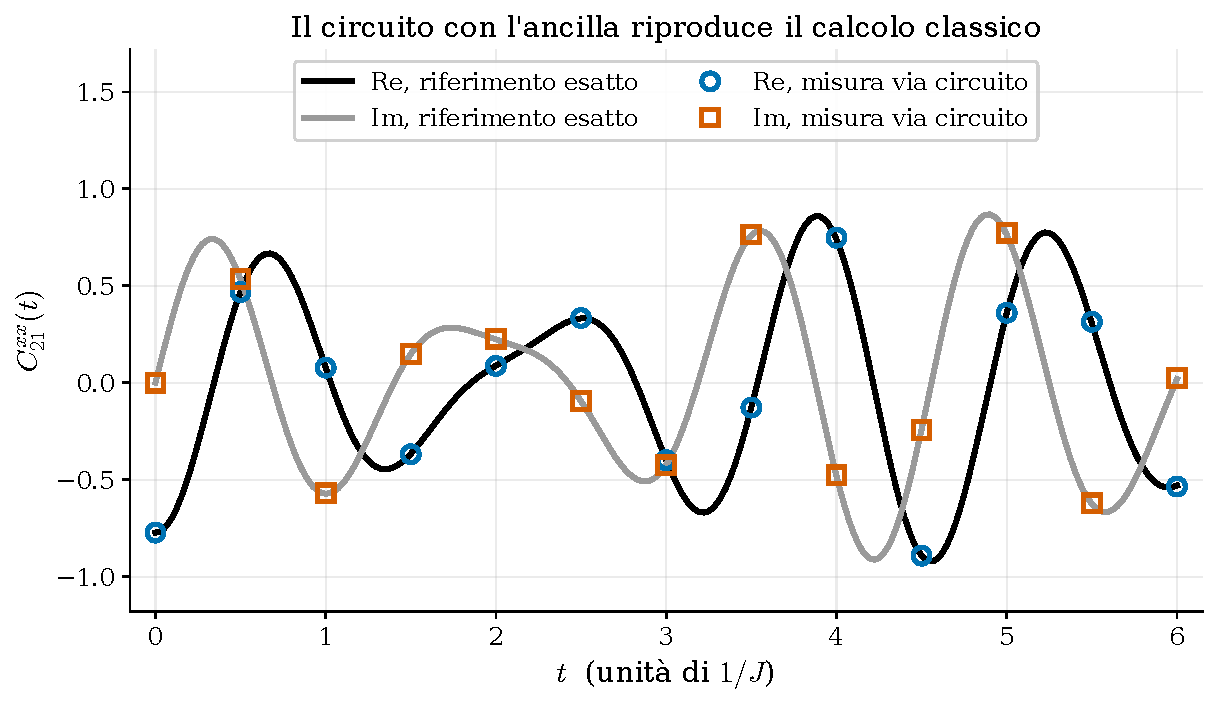
\includegraphics[width=0.86\textwidth]{figure/fig07_correlatore_validazione}
\caption{Un correlatore rappresentativo. Le curve continue sono il riferimento
classico; i simboli sono i valori estratti dal circuito quantistico. I due si
sovrappongono su tutto l'intervallo, per parte reale e parte immaginaria.}
\end{figure}

\FloatBarrier

\verifica{Il riferimento classico non è calcolato con la stessa formula usata
nel circuito, ma con l'esponenziale di matrice diretta: un'implementazione
indipendente, che non condivide codice con la prima. Il residuo medio è
$4.5\times10^{-3}$, il massimo $1.1\times10^{-2}$, con $N=200$ passi di
Trotter; cresce con $t$, come atteso se l'unica sorgente di discrepanza è la
discretizzazione temporale.}

\needspace{8\baselineskip}
\section{Quali combinazioni vale la pena misurare}

Con due siti e tre componenti le combinazioni sono $36$. Non sono equivalenti:
alcune portano un segnale ricco, altre quasi nulla. Vale la pena mapparle tutte
prima di sceglierne una.

\begin{figure}[htbp]
\centering
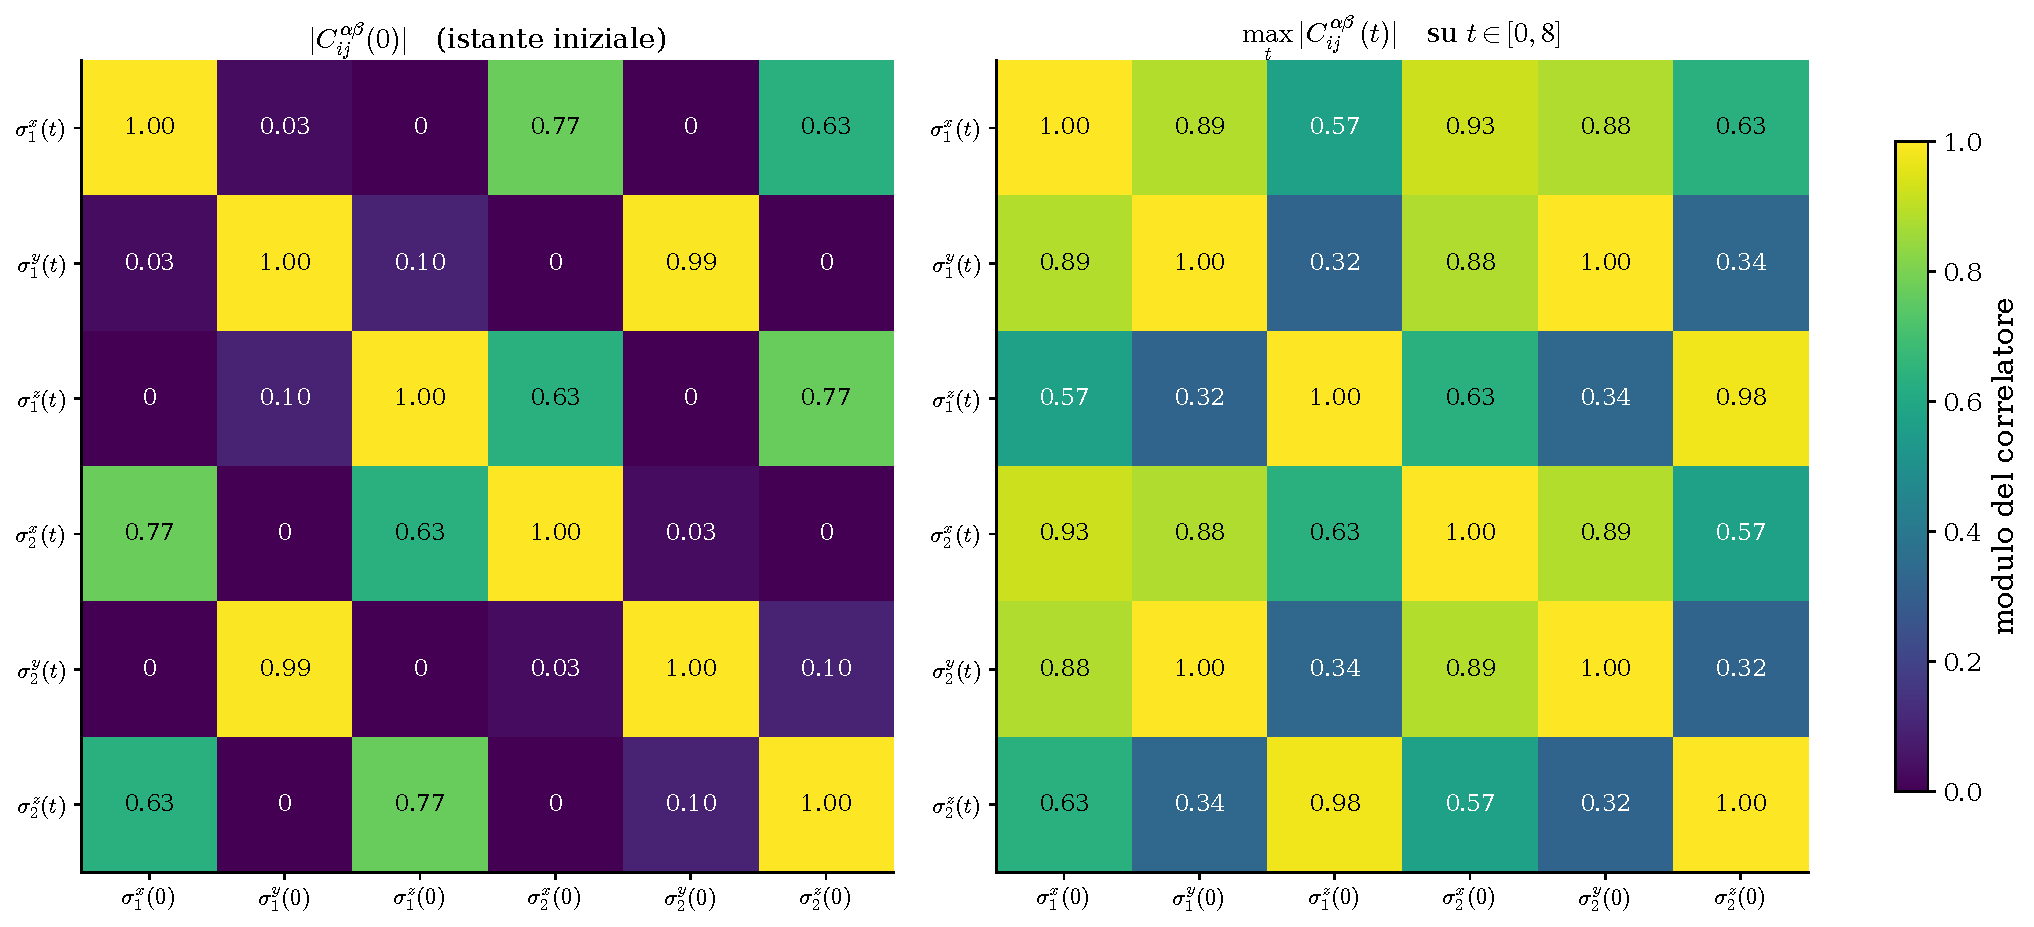
\includegraphics[width=\textwidth]{figure/fig08_scan36}
\caption{Tutte le $36$ combinazioni al punto di lavoro ``test 2''. \textbf{A
sinistra} il valore all'istante iniziale: dodici caselle sono esattamente nulle.
\textbf{A destra} l'ampiezza massima raggiunta nell'intervallo: nessuna casella
è nulla. Il confronto fra i due pannelli è il risultato: gli zeri sono zeri
\emph{iniziali}, non zeri per ogni tempo. Una combinazione che parte da zero può
comunque diventare un buon segnale, e scartarla guardando solo $t=0$ sarebbe un
errore.}
\label{fig:scan}
\end{figure}

\FloatBarrier

Gli zeri del pannello sinistro hanno una spiegazione a una riga, che si può
enunciare senza calcoli. L'Hamiltoniana del dimero è una matrice reale e
simmetrica, quindi il suo
stato fondamentale si può scegliere reale. Ogni prodotto
$\sigma_i^\alpha\sigma_j^\beta$ che risulti hermitiano ma puramente immaginario
ha allora media nulla su uno stato reale. Sono esattamente due famiglie: le
combinazioni a siti diversi con una sola componente $y$ (otto casi) e le
combinazioni sullo stesso sito con componenti $x$ e $z$ (quattro casi).

\verifica{Le dodici caselle nulle sono verificate numericamente a precisione
macchina, e la classificazione appena data le riproduce tutte e dodici, senza
eccezioni e senza casi in più. Il criterio è quindi predittivo, non una lettura
a posteriori della figura.}

\needspace{10\baselineskip}
\section{Ricco e povero: la stessa fisica vista da angoli diversi}

\begin{figure}[htbp]
\centering
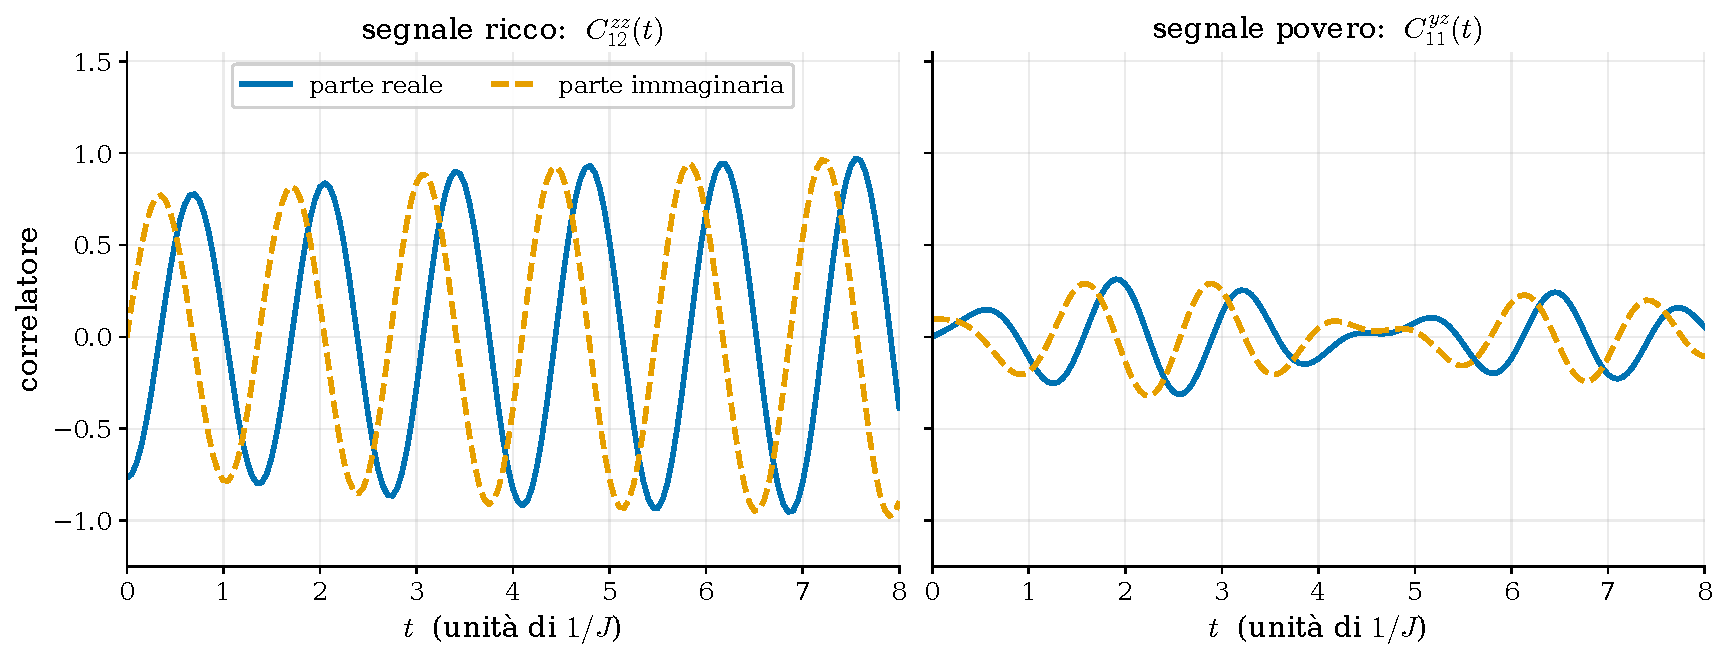
\includegraphics[width=\textwidth]{figure/fig09_ricco_piatto}
\caption{Due correlatori a confronto, sugli stessi assi. A sinistra un segnale
ampio e regolare; a destra un segnale di ampiezza tre volte minore e con
struttura più confusa. Entrambi sono correlatori legittimi dello stesso sistema
nello stesso stato: cambia solo quali componenti di spin si perturbano e si
leggono.}
\end{figure}

\FloatBarrier

La differenza si spiega guardando quali transizioni ciascun correlatore riesce a
eccitare. Vale la pena vederlo esplicitamente, non solo enunciarlo: inserendo
una risoluzione dell'identità nella base degli autostati $\ket{n}$ di $H$
(energie $E_n$, $\ket{0}=\ket{\psi_0}$) fra i due operatori,
\begin{equation}
C_{ij}^{\alpha\beta}(t) = \sum_{n} \underbrace{\bra{0}\sigma_i^\alpha\ket{n}\bra{n}\sigma_j^\beta\ket{0}}_{c_n}\; e^{-i(E_n-E_0)t}.
\end{equation}
Il segnale è dunque \emph{esattamente} una somma di quattro esponenziali
complessi, uno per ciascun autostato $n=0,1,2,3$ (il termine $n=0$ non oscilla:
contribuisce solo alla parte costante). Le grandezze $E_n-E_0$ sono energie,
non frequenze in senso stretto --- ma con $\hbar=1$, la stessa convenzione già
usata per il tempo (in unità di $1/J$), differenza di energia e frequenza
angolare di oscillazione coincidono numericamente: è un'identificazione
esatta, non un abuso di linguaggio. Il peso $c_n$ di ciascuna riga dipende da
quanto bene $\sigma_i^\alpha$ e $\sigma_j^\beta$ collegano il fondamentale a
quel livello --- ed è esattamente ciò che la Fig.~\ref{fig:spettro-righe} più
avanti mostra come istogramma.

\begin{figure}[htbp]
\centering
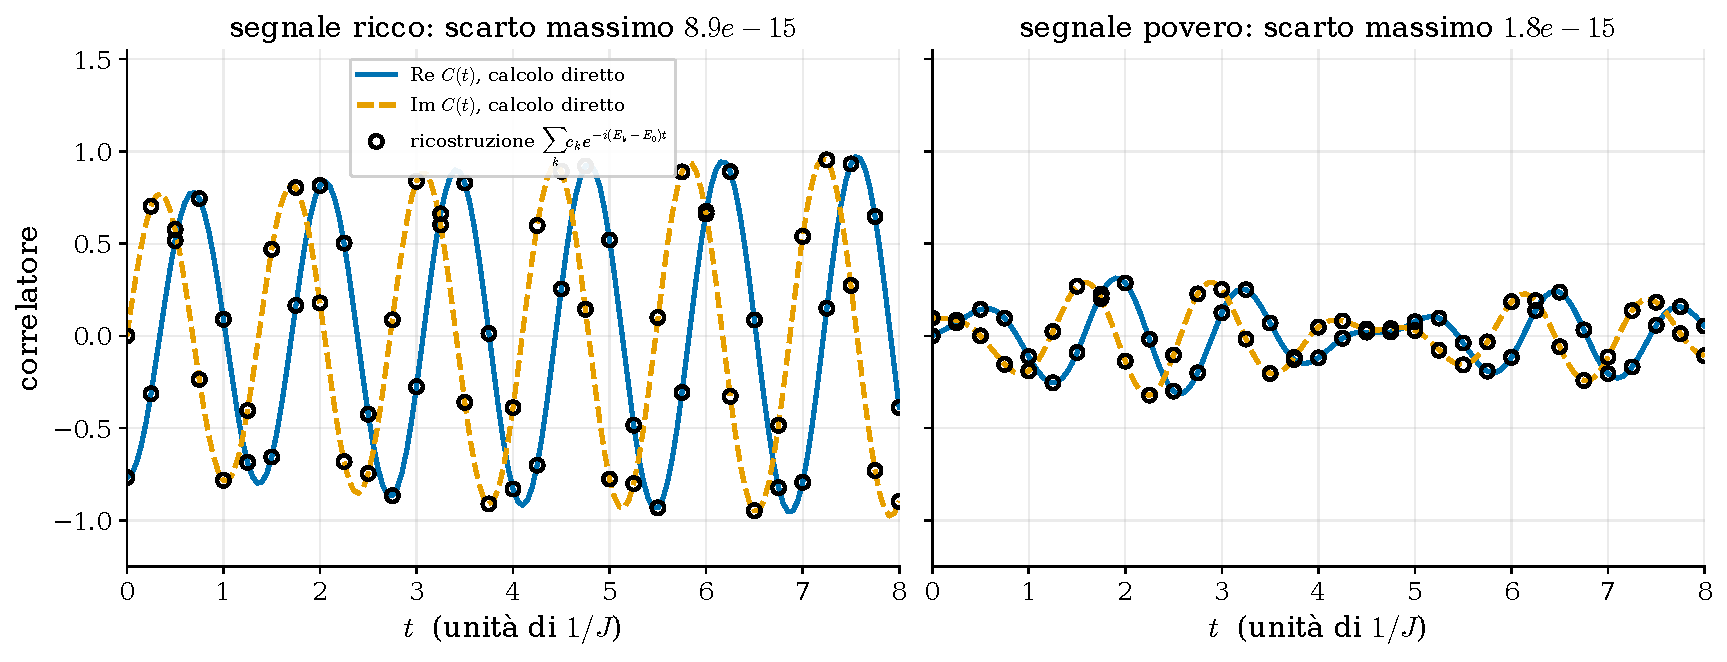
\includegraphics[width=\textwidth]{figure/fig13_ricostruzione_spettrale}
\caption{Verifica diretta della formula: il segnale calcolato nel modo
consueto (linee continue) confrontato con la somma dei quattro esponenziali
$\sum_n c_n e^{-i(E_n-E_0)t}$ ricostruita dai soli autovalori e autovettori di
$H$ (cerchi). Coincidono a precisione macchina --- lo scarto massimo, indicato
nel titolo di ciascun pannello, è dell'ordine di $10^{-14}$--$10^{-15}$: non è
un'approssimazione che funziona bene, è la stessa identità scritta in due
modi.}
\label{fig:ricostruzione-spettrale}
\end{figure}

\FloatBarrier

\begin{figure}[htbp]
\centering
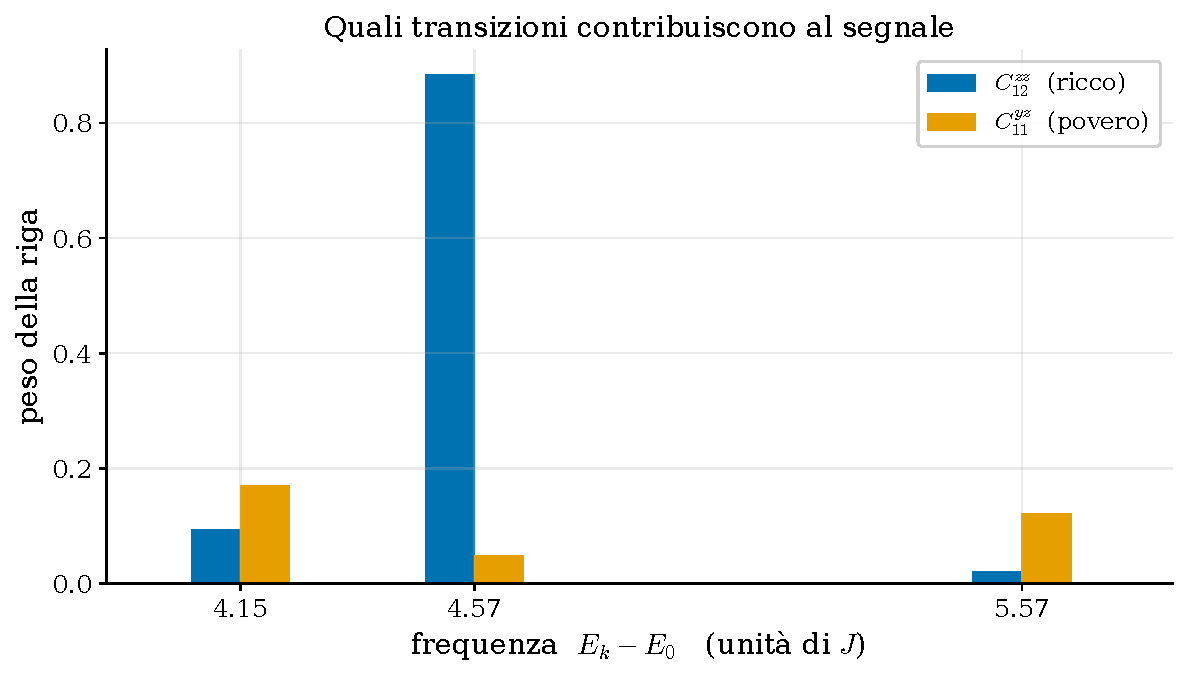
\includegraphics[width=0.76\textwidth]{figure/fig10_spettro_righe}
\caption{Il peso delle tre transizioni disponibili, per i due correlatori della
figura precedente. Quello ``ricco'' concentra quasi tutto il peso su una sola
riga, e infatti oscilla in modo pulito e ampio. Quello ``povero'' distribuisce
poco peso su tutte e tre: il risultato è un'ampiezza piccola e un profilo
irregolare, somma di contributi confrontabili.}
\label{fig:spettro-righe}
\end{figure}

\FloatBarrier

\messaggio{Il correlatore fisicamente più naturale da chiedere e quello che dà
il segnale migliore non coincidono necessariamente. Le due cose vanno tenute
distinte e dichiarate, non risolte scegliendo in silenzio.}

\needspace{10\baselineskip}
\section{Quando la preparazione non è esatta}

Tutto quanto sopra parte dalle ampiezze esatte di $\ket{\psi_0}$. Ma il
Documento 2 ha già costruito due stati di preparazione veri e propri --- quelli
del VQE --- e alla stessa ``test 2'' le loro fidelity sono molto diverse:
$0.9402$ per l'ansatz minimo, $1$ (a sei cifre) per quello esteso. Vale la pena
chiedersi cosa succede al correlatore, non solo alla dinamica del Documento 3,
quando la preparazione parte da lì.

\begin{figure}[htbp]
\centering
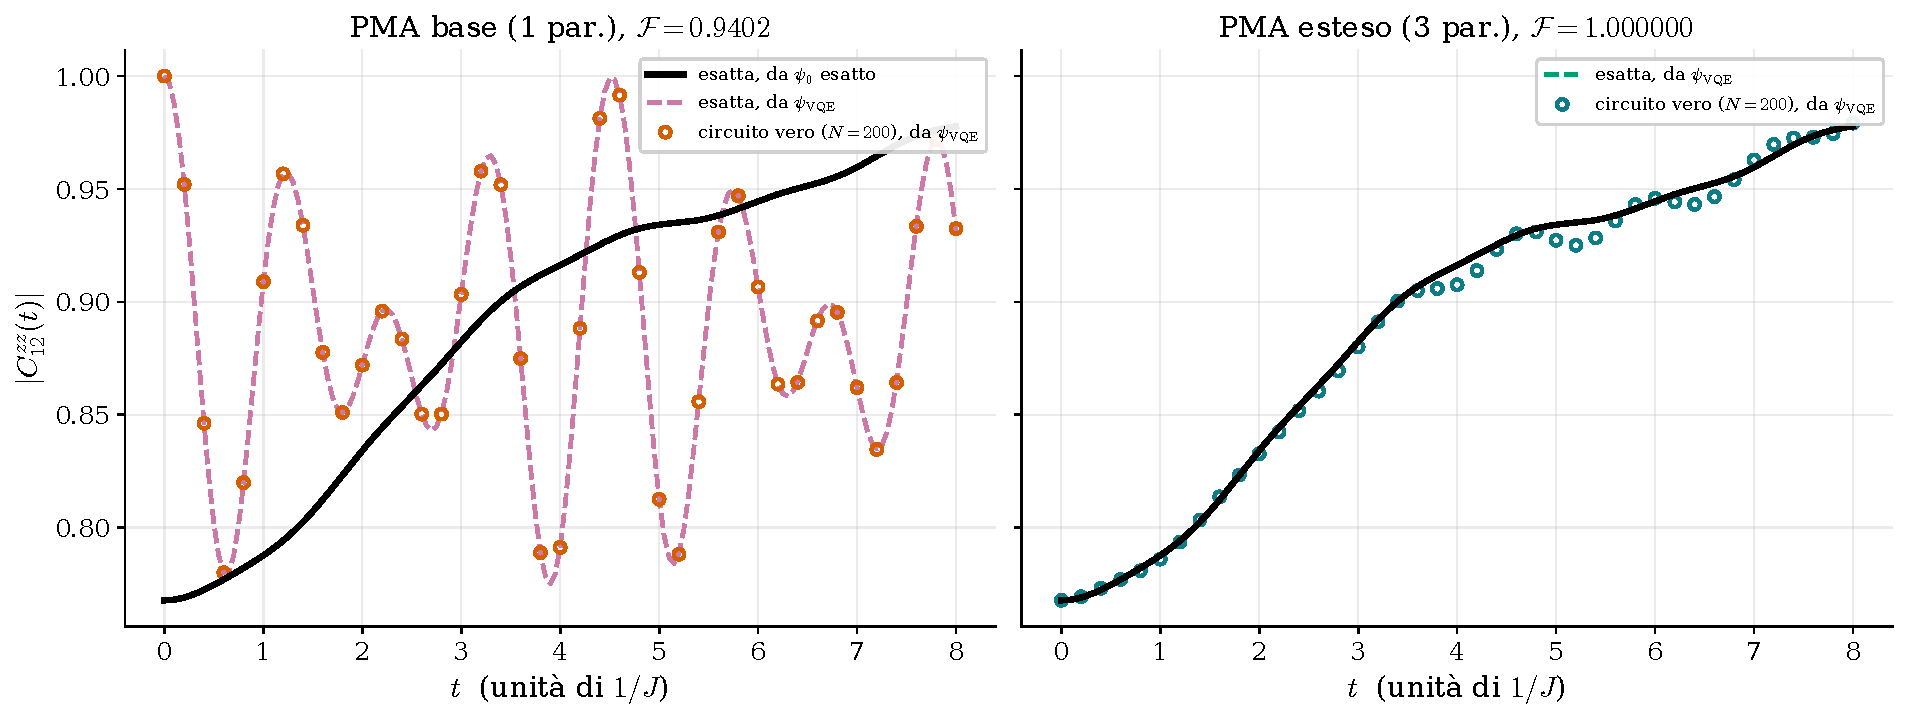
\includegraphics[width=\textwidth]{figure/fig14_correlatore_da_vqe}
\caption{Il correlatore ``ricco'' $C_{12}^{zz}(t)$, in modulo, preparato con
due ansatz diversi del Documento 2 e fatto evolvere con il circuito
completo --- ansatz, ancilla, $N=200$ passi di Trotter, transpilato in porte
native. \textbf{A sinistra}, PMA base: la curva esatta da $\psi_{\rm VQE}$
(viola tratteggiata) e il circuito vero (cerchi) sono quasi indistinguibili
fra loro --- entrambe oscillano con un profilo completamente diverso dal
riferimento esatto (nero): non solo un errore di ampiezza, un errore di
\emph{fase}, coerente con l'aver perso l'accesso a due dei quattro autostati
che contribuiscono alla somma spettrale di
Fig.~\ref{fig:ricostruzione-spettrale}. \textbf{A destra}, PMA esteso: la
curva esatta e il circuito vero sono vicini ma non più identici --- per la
prima volta si vede l'errore di Trotter da solo, non più nascosto da un
esponenziale esatto che un circuito reale non potrebbe realizzare.}
\label{fig:correlatore-vqe}
\end{figure}

\FloatBarrier

Lo scarto massimo su $|C(t)|$, circuito vero incluso, è $0.232$ con l'ansatz
minimo --- identico a prima, perché l'errore di preparazione è talmente più
grande dell'errore di Trotter che quest'ultimo è invisibile nella somma.
Con l'ansatz esteso è $0.010$: non più zero. Prima, usando l'esponenziale
esatto anche per lo stato del VQE, quel numero sarebbe stato $0$ per
costruzione --- un artefatto di aver chiesto al calcolo qualcosa che un
circuito vero non può dare. Con il circuito vero, l'unico errore rimasto è
quello di Trotter, e infatti è dello stesso ordine di grandezza (non
identico: stati diversi hanno contenuto in frequenza diverso) di quello già
misurato per $\langle S_z^{\rm tot}\rangle(t)$ nel Documento 3.
Lo stesso schema già visto per la dinamica: la conclusione non cambia
spostandosi da una grandezza all'altra, l'errore di preparazione, quando
c'è, domina qualunque cosa si stia misurando a valle --- e ora lo dice un
circuito genuinamente eseguito, non più un calcolo che pretendeva di
esserlo.

Un solo correlatore, però, non dice se $C_{12}^{zz}$ sia un caso rappresentativo
o un caso sfortunato. Vale la pena rifare lo scan completo di
Fig.~\ref{fig:scan}, questa volta con lo stato del PMA base al posto delle
ampiezze esatte, su tutte e $36$ le combinazioni:

\begin{figure}[htbp]
\centering
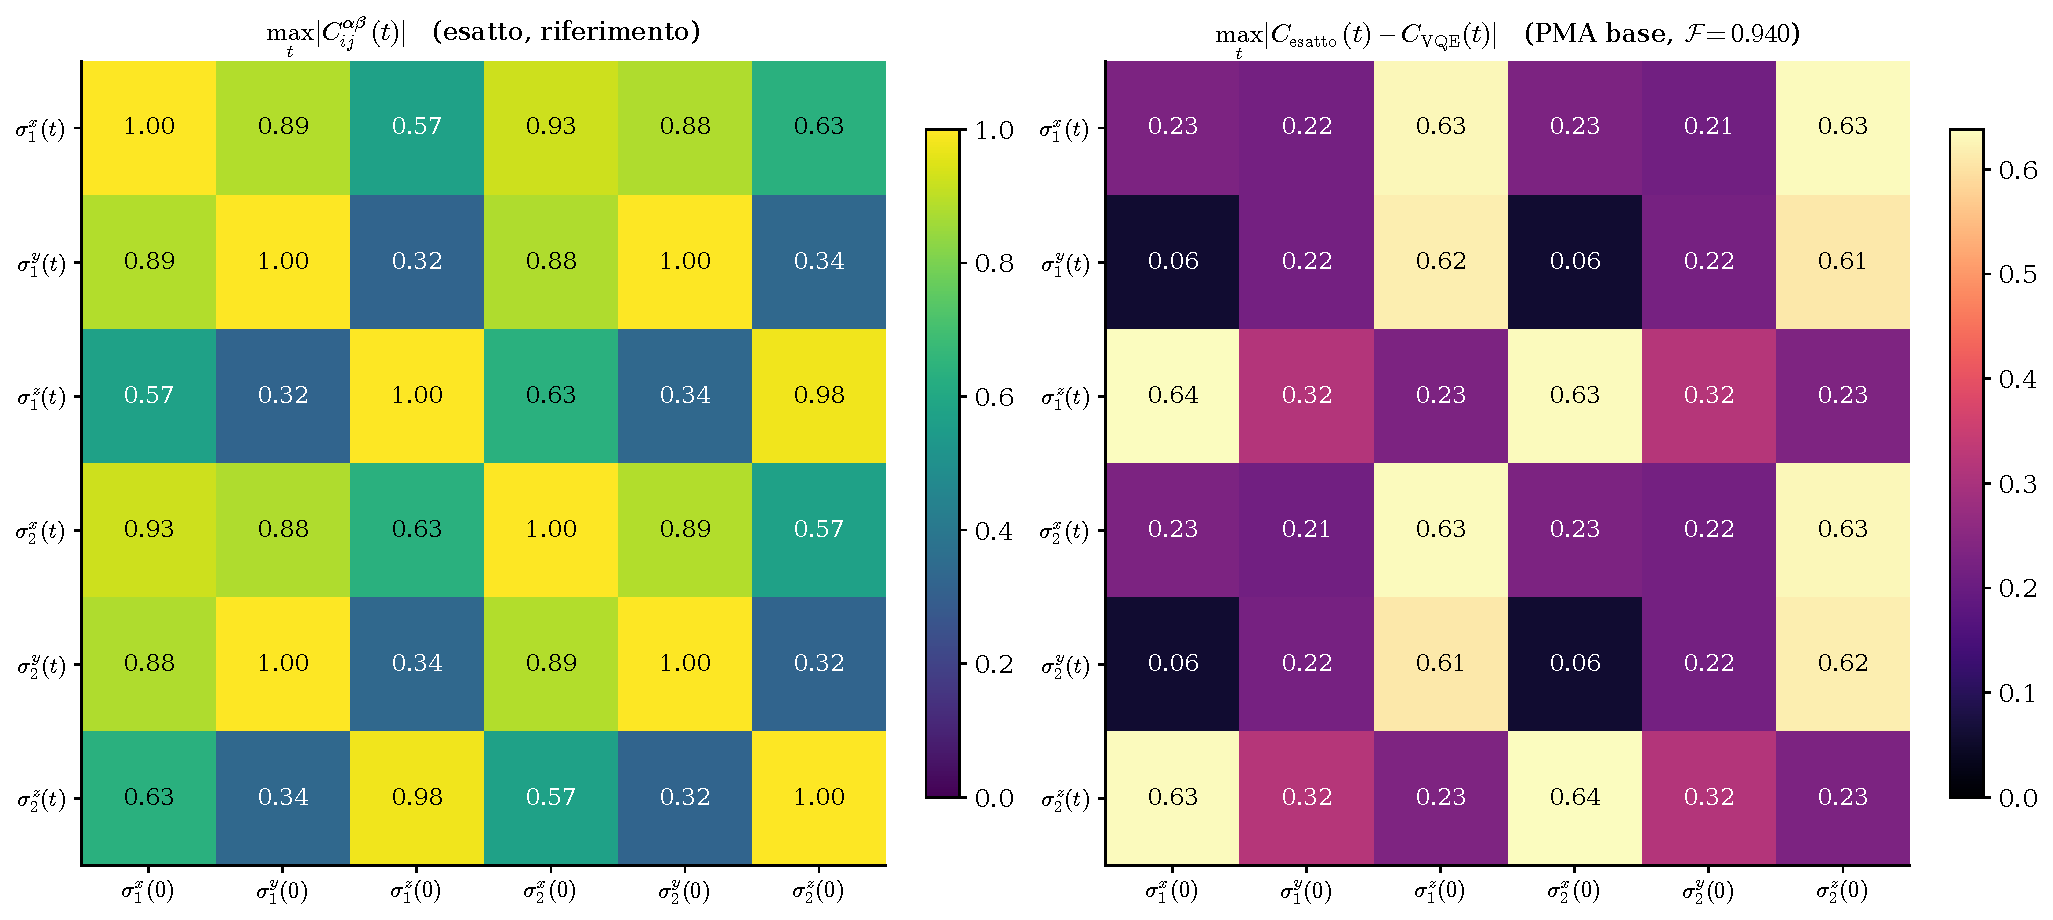
\includegraphics[width=\textwidth]{figure/fig15_scan36_vqe}
\caption{\textbf{A sinistra}, lo stesso riferimento esatto di
Fig.~\ref{fig:scan} (pannello destro), riportato per confronto. \textbf{A
destra}, lo scarto massimo $\max_t|C_{\rm esatto}(t)-C_{\rm VQE}(t)|$ con il
PMA base come preparazione, sulle stesse $36$ combinazioni. Il pattern non è
uniforme: le combinazioni con una componente $y$ affiancata a una $x$ (per
esempio $\sigma_1^y$--$\sigma_1^x$ o $\sigma_2^y$--$\sigma_2^x$) restano quasi
indenni (scarto $\approx0.06$), mentre qualunque combinazione che coinvolge una
componente $z$ soffre molto di più (scarto fra $0.32$ e $0.64$) --- coerente
con la struttura del blocco CNOT--$R_y$--CNOT dell'ansatz minimo (Documento 2,
Fig.~3), che agisce con una rotazione attorno a $y$ e quindi lascia quella
direzione relativamente protetta.}
\label{fig:scan-vqe}
\end{figure}

\FloatBarrier

Lo scarto medio sulle $36$ combinazioni è $0.35$, con un fattore
$10\times$ fra la combinazione più robusta ($0.06$) e la più fragile ($0.64$).
Il correlatore $C_{12}^{zz}$ scelto come esempio in Fig.~\ref{fig:correlatore-vqe}
non era un caso pessimo isolato: è vicino alla parte alta della distribuzione,
ma non ne è l'estremo. La chiusura è ora sistematica su questo punto
specifico --- resta aperto, come dichiarato nella sezione seguente, verificare
lo stesso effetto passando dal calcolo classico usato qui al circuito
quantistico vero con l'ancilla.

\messaggio{L'imperfezione del VQE non pesa allo stesso modo su tutti i
correlatori: alcune direzioni di spin restano protette dalla struttura stessa
dell'ansatz, altre no. Sceglierne uno "a caso" per riportare l'esito di un
esperimento sarebbe fuorviante quanto scegliere il più comodo da misurare
(Fig.~\ref{fig:spettro-righe}) senza dichiararlo.}

\section{Che cosa manca, dichiarato}

Tutto quanto sopra è a simulazione ideale. In particolare:

\begin{itemize}[leftmargin=1.5em,itemsep=2pt]
\item L'ancilla è letta sul vettore di stato esatto: non c'è rumore statistico
da numero finito di ripetizioni, né errore di lettura.
\item Non c'è rumore di gate, e il circuito dei correlatori è il più lungo di
tutto il progetto --- contiene $N$ passi di Trotter più le porte controllate.
È quindi il candidato naturale come primo banco di prova quando si introdurrà
il rumore.
\item La preparazione dello stato iniziale, in tutto il documento tranne la
sezione precedente, usa le ampiezze esatte, non il circuito VQE del
Documento 2. La sezione precedente usa il circuito vero (ansatz $+$ ancilla
$+$ Trotter) per il correlatore singolo di
Fig.~\ref{fig:correlatore-vqe}; lo scan sistematico sulle $36$ combinazioni
(Fig.~\ref{fig:scan-vqe}) resta invece sul calcolo diretto, per motivi di
tempo di calcolo --- verificare lo stesso scan con il circuito completo su
tutte e $36$ le combinazioni resta aperto. Per le due topologie a $N=3$
questa chiusura, circuito incluso, è già stata fatta e validata.
\end{itemize}

\end{document}
